\documentclass[10pt,a4 paper,landscape]{article}
% -- Layout ----
\usepackage[top=0.6cm, bottom=0.6cm, left=0.5cm, right=0.5cm, landscape]{geometry}

% -- Titles ----
\usepackage[
  tiny,                     % text size title
  compact                   % reduce vertical space before/after title
]{titlesec}
% \titlespacing*
\titleformat{\section}{\normalfont\small\bfseries}{\thesection}{0em}{} % Remove space before and after section titles
\titleformat{\subsection}{\normalfont\small\bfseries}{\thesubsection}{0em}{} % Remove space before and after subsection titles
\titlespacing*{\section}{0pt}{0pt}{0pt} % Remove space before/after section titles
\titlespacing*{\subsection}{0pt}{0pt}{0pt} % Remove space before/after subsec titles

% -- Colors ----
\usepackage[dvipsnames]{xcolor}
\definecolor{dmm}{RGB}{192,192,192} % Define a custom dimmed text color
\definecolor{cmt}{RGB}{61,123,123}

% -- Math ------
\usepackage{mathtools}
\usepackage{amssymb}
\usepackage{turnstile}%better vdash

% -- Lists -----
\usepackage[inline]{enumitem}
\setlist{noitemsep}% Remove vspace between items
% Set vspace before and after  list environments as well as the left margin
\setlist[itemize,1]{leftmargin=.6em,labelindent=0pt,labelsep=2pt,
  topsep=1pt,partopsep=1pt}
\setlist[enumerate,1]{leftmargin=1em,labelindent=0pt,labelsep=2pt,
  topsep=1pt,partopsep=1pt}
\setlist[itemize,2]{leftmargin=.3em,labelindent=1pt,topsep=1pt,partopsep=1pt}
\setlist[enumerate,2]{leftmargin=0.2em,labelindent=1pt,topsep=1pt,partopsep=1pt}
\setlist[description]{labelwidth=\linewidth,font=\small\bfseries,leftmargin=1em,topsep=1pt,partopsep=1pt}
% -- Code listing ---
\usepackage{listings}
\lstset{
  aboveskip=3pt,
  belowskip=3pt,
  basicstyle=\small\ttfamily,
  breaklines=true,
  % commentstyle=\upshape\ttfamily,
  captionpos=b,
  commentstyle=\color{cmt},
  frame=single,
  keepspaces=false,
  keywordstyle=\bfseries,
  showspaces=false,
  showstringspaces=false,
  showtabs=false,
  tabsize=2,
}

% Parse Trees
\usepackage{tikz}
\usetikzlibrary{ arrows, automata, bbox, calc, positioning,  decorations.pathmorphing, decorations.pathreplacing, decorations.shapes, }
\tikzset{
% ->, % makes the edges directed
>=stealth', % makes the arrow heads bold
node distance=1cm, % specifies minimum distance between two nodes
% small/.style={},
every state/.style={thick}, % sets the properties for each ’state’ node
every node/.style={inner sep=1pt},
initial text=start, % sets the text that appears on the start arrow
}

% Place a figure env right here via [H] option
\usepackage{float}

% Side by side figure
\usepackage{subcaption}
% \usepackage{caption}
% \captionsetup{belowskip=0pt, aboveskip=0pt}


% -- Multi-Col layout --
\usepackage{multicol}

% No indentation
\setlength\parindent{0pt}
\setlength\abovedisplayskip{-5pt}
\setlength\belowdisplayskip{-5pt}
\setlength\abovedisplayshortskip{-4pt}
\setlength\belowdisplayshortskip{-4pt}
\newcommand{\gor}{\;|\;}
\newcommand{\num}{\texttt{\#}~}
\renewcommand{\arraystretch}{1.2}


\lstset{
  numberstyle=\ttfamily\footnotesize,
}
\begin{document}
% Suppress page number for all pages
\pagestyle{empty}
% Each section goes into this env
\begin{multicols*}{2}
% \section*{Predictive parsing - LL(1) and its parse table}
\begin{align*}
  E \to\;& E + T \gor T         \tag{1} \\
  T \to\;& T * F \gor F         \tag{2} \\
  F \to\;& (E) \gor \mathsf{id} \tag{3}
\end{align*}
\section*{Step 1: Eliminate left recursion (if any or skip if none)}
\begin{align*}
  E\,  & \to\; TE'                     \tag{1} \\
  E'\, & \to\; +\,TE' \gor \varepsilon \tag{2} \\
  T\,  & \to\; FT'                     \tag{3} \\
  T'\, & \to\; *\,FT' \gor \varepsilon \tag{4} \\
  F\,  & \to\; (E)    \gor \mathsf{id} \tag{5}
\end{align*}
\section*{Step 2: Remove common prefix by left factoring}
\mb{NO} common prefix shared by any 2 productions, so skip

\section*{Step 3: Collect FIRST and FOLLOW sets}
\begin{itemize}
\item \mo{FIRST} set for each production
  \begin{align*}
    \mfn{first}(E)  &= \mfn{first}(T) = \mfn{first}(F) \\
                    &= \mfn{first}(() \cup \mfn{first}(\mathsf{id})
                      = \mset{\left(\right.,\mathsf{id}} \\
    \mfn{first}(E') &= \mfn{first}(+)\cup\mfn{first}(\varepsilon)
                      = \mset{+,\varepsilon}                  \\
    \mfn{first}(T)  &= \mfn{first}(F) = \mset{(,\mathsf{id}}  \\
    \mfn{first}(T') &= \mfn{first}(*)\cup\mfn{first}(\varepsilon)
                      = \mset{*,\varepsilon}  \\
    \mfn{first}(F)  &= \mfn{first}(()\cup\mfn{first}(\mathsf{id})
                      = \mset{(,\mathsf{id}}
  \end{align*}
\item \mo{FOLLOW} set for each production (include \$(\texttt{EOF}))
  \begin{align*}
    \mfn{follow}(E)  &= \mfn{first}()) = \mset{)} \Rightarrow \mset{), \$}     \\
    \mfn{follow}(E') &= \mfn{follow}(E) = \mset{), \$} \Rightarrow \mset{), \$}\\
    \mfn{follow}(T)  &= \mfn{first}(E')\cup\mfn{follow}(E')\cup\mfn{follow(E)} \\
                     &= \mset{+, \left.\right), \$} \\
    \mfn{follow}(T') &= \mfn{follow}(T) = \mset{+, ), \$}\\
    \mfn{follow}(F)  &= \mfn{first}(T')\cup\mfn{follow}(T)= \mset{*, +, ), \$}
    \end{align*}
  \item summary table of \mo{FIRST} and \mo{FOLLOW} sets
    \begin{center}
      \begin{tabular}{l|l|r}
        \hline
        N  & \textsf{FIRST} & \textsf{FOLLOW} \\
        \hline
        \(E\)   & \(\mset{(,\mathsf{id}}\) & \(\mset{), \$}\) \\
        \(E'\)  & \(\mset{+,\varepsilon}\) & \(\mset{), \$}\) \\
        \(T\)   & \(\mset{(,\mathsf{id}}\) & \(\mset{+, ), \$}\) \\
        \(T'\)  & \(\mset{*,\varepsilon}\) & \(\mset{+, ), \$}\) \\
        \(F\)   & \(\mset{(,\mathsf{id}}\) & \(\mset{*, +, ), \$}\) \\
        \hline
      \end{tabular}
  \end{center}
\end{itemize}


\section*{Step 4: LL(1) parse table}
\begin{enumerate}
\item For \mb{non-$\varepsilon$} productions, use \mo{\textsf{FIRST}(RHS)} to locate cols and put production or production number there
  \begin{align*}
    \mfn{first}(RHS_{E}) &=\mfn{first}(TE')=\mfn{first}(T) = \mset{(,\mathsf{id}} \\
    \mfn{first}(RHS_{E'})&=\mfn{first}(+TE')=\mfn{first}(+) = \mset{+} \\
    \mfn{first}(RHS_{T}) &=\mfn{first}(FT')=\mfn{first}(F) = \mset{(,\mathsf{id}} \\
    \mfn{first}(RHS_{T'})&=\mfn{first}(*FT')=\mfn{first}(*) = \mset{*} \\
    \mfn{first}(RHS_{F}) &=\mfn{first}((E))= \mfn{first}(() = \mset{(} \\
    \mfn{first}(RHS_{F}) &=\mfn{first}(\mathsf{id}) = \mset{\mathsf{id}}
  \end{align*}
  \begin{tabular}{l|c|c|c|c|c|c}
  \hline
  N       & +          & id  & *          & (           & )   & \$(\texttt{EOF})\\
  \hline
  \(E\)   &            &\(\to TE'\)&& \(\to TE'\) &     & \\
  \(E'\)  &\(\to +TE'\)& &&&\\
  \(T\)   &            &\(\to FT'\)    &            &\(\to FT'\) &\\
  \(T'\)  &            &      &\(\to *FT'\)&&\\
  \(F\)   &            &\(\to \mathsf{id}\)& &\(\to (E)\)&&\\
  \hline
  \multicolumn{7}{l}{rows: non-terminals (LHS); cols: terminals; entry: RHS}\\
  \hline
  \multicolumn{7}{l}{can also use production number for each entry}\\
  \hline
  \end{tabular}
\vspace{.1em}
\item For \mb{$\boldsymbol{\varepsilon}$} productions, use \mo{\textsf{FOLLOW}(LHS)} to locate cols and put \mb{$\boldsymbol{\varepsilon}$} there
  \begin{align*}
    \mfn{follow}(LHS_{E'})&= \mset{), \$}\\
    \mfn{follow}(LHS_{T'})&= \mset{+, ), \$}
  \end{align*}
  \begin{tabular}{l|c|c|c|c|c|c}
  \hline
  N       & +          & id  & *          & (           & )   & \$(\texttt{EOF})\\
  \hline
  \(E\)   &            &\(\to TE'\)&      & \(\to TE'\) && \\
  \(E'\)  &\(\to +TE'\)&     &            &  &\(\varepsilon\) &\(\varepsilon\)\\
  \(T\)   &            &\(\to FT'\)    &                &\(\to FT'\) &\\
  \(T'\)  &\(\varepsilon\) & &\(\to *FT'\)&  &\(\varepsilon\)&\(\varepsilon\)\\
  \(F\)   &            &\(\to \mathsf{id}\)& &\(\to (E)\)&&\\
  \hline
  \multicolumn{7}{l}{rows: non-terminals (LHS); cols: terminals; entry: RHS}\\
  \hline
  \multicolumn{7}{l}{can also use production number for each entry}\\
  \hline
  \end{tabular}
\end{enumerate}
\begin{itemize}
\item If the grammar includes minus \mb{-}, it will be the same as \mb{+}
\item if the grammar includes division \mb{$\boldsymbol{\backslash}$}, it will be the same as \mb{*}
\item if the grammar includes a start symbol $S\to E\$$
  \begin{center}
  \begin{tabular}{l|l|l}
    \hline
    N      & \textsf{FIRST} & \textsf{FOLLOW} (empty) \\
    \hline
    \(S\)  & \(\mset{(,\mathsf{id}}\) & \\
    \hline
    \multicolumn{3}{l}{FIRST same as $E$, FOLLOW is empty}\\
    \hline
  \end{tabular}\\
  \begin{tabular}{l|c|c|c|c|c|c}
  \hline
  N       & +          & id  & *          & (           & )   & \$(\texttt{EOF})\\
  \hline
  \(S\)   &            &\(\to E\$\)&      & \(\to E\$\) && \\
  \hline
  \end{tabular}
  \end{center}
\end{itemize}
\section*{LL (1) parsing example (suppose stack top is the left end)}
\begin{enumerate}
\item \mb{Update stack} stack top is a non-terminal; try to replace it with RHS of its production(s)
\item \mb{Input match} stack top is terminal; match with current input symbol; remove the symbol from input; pop stack
\item \mb{Accept}: stack = input buffer = \$
\item \mb{Error}: when there is a mismatch, throws error
\end{enumerate}
\begin{minipage}{\linewidth}
\centering
\begin{tabular}{l|l|l|l}
  \hline
  Stack & Input buffer                          & Action  & Use Production  \\
  \hline
  $E\$$ & $\mathsf{id}*\mathsf{id}+\mathsf{id}\$$ & Update stack & $E\to TE'$\\
  $TE'\$$ & $\mathsf{id}*\mathsf{id}+\mathsf{id}\$$ & Update stack &$T\to FT'$\\
  $FT'E'\$$ & $\mathsf{id}*\mathsf{id}+\mathsf{id}\$$ & Update stack$^{\mr{1}}$ &$F\to \mathsf{id}$\\
  $\mathsf{id}T'E'\$$ & $\mathsf{id}*\mathsf{id}+\mathsf{id}\$$ & Match &\\
  $T'E'\$$ & $*\mathsf{id}+\mathsf{id}\$$ & Update stack$^{\mr{2}}$ & $T'\to *FT'$\\
  $*FT'E'\$$ & $*\mathsf{id}+\mathsf{id}\$$ & Match & \\
  $FT'E'\$$ & $\mathsf{id}+\mathsf{id}\$$ & Update stack &$F\to \mathsf{id}$ \\
  $\mathsf{id}T'E'\$$ & $\mathsf{id}+\mathsf{id}\$$ & Match & \\
  $T'E'\$$ & $+\mathsf{id}\$$ & Update stack$^{\mr{3}}$ & $T'\to \varepsilon$\\
  $E'\$$ & $+\mathsf{id}\$$ & Update stack & $E'\to +TE'$\\
  $+TE'\$$ & $+\mathsf{id}\$$ & Match & \\
  $TE'\$$ & $\mathsf{id}\$$ & Update stack & $T\to FT'$\\
  $FT'E'\$$ & $\mathsf{id}\$$ & Update stack & $F\to \mathsf{id}$\\
  $\mathsf{id}T'E'\$$ & $\mathsf{id}\$$ & Match & \\
  $T'E'\$$ & $\$$ & Update stack & $T'\to \varepsilon$ \\
  $E'\$$ & $\$$ & Update stack & $E'\to \varepsilon$ \\
  $\$$ & $\$$ & Accept &  \\
  \hline
  \multicolumn{4}{l}{\mr{1}: LL(1) parser knows $F\to \mathsf{id}$ if it sees \textsf{id} ahead}\\
  \hline
  \multicolumn{4}{l}{\mr{2}: LL(1) parser knows $T'\to *FT'$ if it sees \textsf{*} ahead}\\
  \hline
  \multicolumn{4}{l}{\mr{3}: LL(1) parser knows $T'\to \varepsilon$ if it sees other stuff ahead}\\
  \hline
\end{tabular}
\end{minipage}
\begin{itemize}
\item \textbf{Use Prod.} shows the leftmost derivation and parse tree
  \begin{center}
    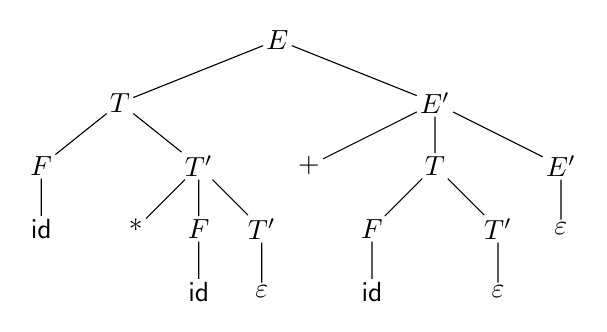
\begin{tikzpicture}[level distance=8mm]
      \node {$E$}
      [sibling distance=40mm]
      child {
        node {$T$}
        [sibling distance=20mm]
        child {
          node {$F$} child { node {\mr{$\mathsf{id}$}} }
        }
        child {
          node {$T'$}
          [sibling distance=8mm]
          child  {node {\mr{*}}}
          child  {node {$F$} child {node {\mr{$\mathsf{id}$}}}}
          child  {node {$T'$} child {node {\mr{$\varepsilon$}}}}
        }
      }
      child {
        node {$E'$}
        [sibling distance=16mm]
        child  {node {\mr{+}}}
        child  {
          node {$T$}
          child {node {$F$} child {node {\mr{$\mathsf{id}$}}}}
          child {node {$T'$} child {node {\mr{$\varepsilon$}}}}
        }
        child  {node {$E'$} child {node {\mr{$\varepsilon$}}}}
      };
    \end{tikzpicture}
    \end{center}
\item leaf nodes from left to right build the original input string
\[\mathsf{id} * \mathsf{id} + \mathsf{id} \]
\end{itemize}

% \input{sec/LR0}
% \section*{Conflicts in LR parsing}
\begin{itemize}
\item \mb{shift} the dot past the input symbol currently before the dot
\item[] Before: $X\to \lrd A\beta$; After: $X\to A\lrd\beta$
\item \mb{reduce}: when dot at the end of item, RHS of the production can be replaced with the LHS
\item In a state $I$, expect to have either a reduce or a shift action, not both. Otherwise, there is a \mo{conflict}:
  \begin{enumerate}
  \item \mb{S}/\mb{R} conflict: state $I$ has a reduce \textbf{AND} a shift action
  \item \mb{R}/\mb{R} conflict: state $I$ has two reduce actions
  \end{enumerate}
\end{itemize}
\section*{Example: A grammar with S/R conflict}
\begin{minipage}{.5\linewidth}
\begin{align*}
  _0\quad S&\to E\$   \\
  _1\quad E&\to T + E
\end{align*}
\end{minipage}
\begin{minipage}{.5\linewidth}
\begin{align*}
  _2\quad E&\to T \\
  _3\quad T&\to x
\end{align*}
\end{minipage}
\section*{grammar DFA with R/S conflict}
\begin{tikzpicture}
  % I1
  \node (i1) [lrst, anchor=north east] {
    $S\to \lrd E\$$\\
    $E\to \lrd T + E$\\
    $E\to \lrd T$\\
    $T\to \lrd x$
  };
  \node [above=1mm of i1.north east, font=\footnotesize\bf]{1};

  %I2
  \node (i2) [lrst, right=12mm of i1.north east, anchor=north west] {
    $S\to E\lrd\$$
  };
  \node (m2) [above=1mm of i2.north east, font=\footnotesize\bf]{2};

  %I3
  \node (i3) [lrst, right=12mm of i1.east, anchor=north west] {
    $E\to T\lrd + E$\\
    $E\to T\lrd $
  };
  \node (m3) [right=1mm of i3.north east, font=\footnotesize\bf]{3};

  %I5
  \node (i5) [lrst, below=15mm of i1.south, anchor=north] {
    $T\to x\lrd$
  };
  \node (m5) [above=1mm of i5.north east, font=\footnotesize\bf]{5};

  %I4
  \node (i4) [lrst, below=6mm of i3, anchor=north] {
    $E\to T + \lrd E$\\
    $E\to \lrd T$\\
    $E\to \lrd T + E$ \\
    $T\to \lrd x$
  };
  \node (m4) [right=1mm of i4.north east, font=\footnotesize\bf]{4};

  %I6
  \node (i6) [lrst, right=10mm of i4, anchor=west] {
    $E\to T + E\lrd$
  };
  \node (m6) [above=1mm of i6.north east, font=\footnotesize\bf]{6};

  % note
  \node(note)[right=8mm of i3.north east, anchor=west, text width=3cm, font=\small] {
    In $I_3$, there are a shift action (over $+$) and a reduce action (dot at the end) $\to$ a S/R conflict in $I_3$ and the grammar is \mr{not} LR(0)
  };

  % paths
  \draw[->] (i1.east |- i2.west) -- (i2.west) node[midway, above]{$E$}  ;
  \draw[->] (i1.mid east |- i3.west) -- (i3.west) node[midway, above]{$T$}  ;
  \draw[->] (i1) edge node[left]{$x$} (i5) ;
  \draw[->]
  ([xshift=4mm]i3.south) -- ([xshift=4mm]i4.north) node[midway,right] {$+$};
  \draw[->]
  ([xshift=-4mm]i4.north) -- ([xshift=-4mm]i3.south) node[midway,left] {$T$};
  \draw[->] (i4) edge node[above]{$E$} (i6);
  \draw[->] (i4.west |- i5.east) -- (i5.east) node[midway, above]{$x$};

\end{tikzpicture}
\section*{Grammar parse table with R/S conflict}
\begin{minipage}{.7\linewidth}
\begin{center}
\begin{tabular}{l|lll|ll}
  State &\multicolumn{3}{c}{Action$^1$} & \multicolumn{2}{c}{Goto$^2$}  \\
  \hline
  $I$ & + & $x$  &\$       & $T$ & $E$  \\
  \hline
   1  &   & $s5$ &         &$g3$& $g2$ \\
   2  &   &      &$a$      && \\
   3  &$s4,r2$&$r2$&$r2$   && \\
   4  &   &$s5$&           &$g3$&$g6$ \\
   5  &$r3$&$r3$&$r3$      &    & \\
   6  &$r1$&$r1$&$r1$      &    & \\
  \hline
  \multicolumn{6}{l}{\footnotesize 1: Action (s/r) only on terminals and \$}\\
  \hline
  \multicolumn{6}{l}{\footnotesize 2: Goto only on non-terminals}\\
  \hline
\end{tabular}
\end{center}
\end{minipage}
\begin{minipage}{.3\linewidth}
  {\small
    In state 3, on symbol +, there is a duplicate entry: The parser must shift
    into state 4 and also reduce by production 2. This is a conflict and indicates
    that the grammar is \mr{not} LR(0).
  }
\end{minipage}
\section*{Use FOLLOW to build SLR and remove S/R conflict}
\begin{enumerate}
\item in each state $I$, identify all the reduce items like $A\to \alpha\lrd$ (dot at the end) where $\alpha \in \Sigma$ (terminals plus \$).
  \begin{itemize}
  \item In $I_2$, $S\to E\lrd\$$, need  $\mfn{follow}(S)$
  \item In $I_3$, $E\to T\lrd$, need $\mfn{follow}(E)$
  \item In $I_5$, $T\to x\lrd$, need $\mfn{follow}(T)$
  \item In $I_6$, $E\to T + E\lrd$, need $\mfn{follow}(E)$
  \end{itemize}
\item for each reduce item above, compute \textsf{FOLLOW}(LHS)
  \begin{itemize}
  \item $\mfn{follow}(S) = \mset{\$}$ (just init the set to include \$)
  \item $\mfn{follow}(T) = \mfn{follow}(E) \cup \mfn{first}(+) = \mset{+,\$}$
  \item $\mfn{follow}(E) = \mset{\$}$
  \end{itemize}
\item for each token $X$ in each computed follow set above, put a reduce action $(I, X, A\to \alpha)$ (on lookahead $X$, reduce by rule $A\to \alpha$) in SLR table
  \begin{itemize}
  \item $(I_2, \$, S\to E\$)$, put $a$ ($r0$) at $(I_2, \$)$
  \item $(I_3, \$, E\to T)$, put $r2$ at $(I_3, \$)$
  \item $(I_5, +, T\to x)$, put $r3$ at $(I_5, +)$
  \item $(I_5, \$, T\to x)$, put $r3$ at $(I_5, \$)$
  \item $(I_6, \$, E\to T + E)$, put $r1$ at $(I_6, \$)$
  \end{itemize}
\end{enumerate}
\begin{center}
\begin{tabular}{l|lll|ll}
  State &\multicolumn{3}{c}{Action} & \multicolumn{2}{c}{Goto}  \\
  \hline
  $I$ & + & $x$  &\$       & $T$ & $E$  \\
  \hline
   1  &   & $s5$ &         &$g3$& $g2$ \\
   2  &   &      &$a$      &    & \\
   3  &$s4$&     &$r2$     && \\
   4  &   &$s5$&           &$g3$&$g6$ \\
   5  &$r3$&&$r3$          &    & \\
   6  &    &    &$r1$      &    & \\
  \hline
\end{tabular}
\end{center}

\section*{LR(1) items $(A\to \alpha\lrd\beta, x)$ with 3 parts; closure, goto}
\begin{itemize}
\item a grammar production: $A\to\ldots$
\item a right-hand-side position (represent by the \mr{dot} $\lrd$)
\item a lookahead symbol $(A\to \alpha\lrd\beta, \mo{x})$
\item The idea is that an item $(A\to\alpha\beta\lrd,x)$ indicates that
  \begin{itemize}
  \item the sequence $\alpha$ is on top of the stack
  \item at the head of the input is a string derivable from $\beta x$
  \end{itemize}
\item $\beta$ can be terminal or non-terminal, $x$ can be $\$$(\texttt{EOF})
\item In pseudo code, $X$ in item $(A\to \alpha\lrd X\beta, z)$ is non-terminal
\end{itemize}
\includegraphics*[width=\linewidth]{img/LR1_closure_goto}
\section*{Example: A LR(1) grammar and its parsing table}
\begin{minipage}{.5\linewidth}
\begin{align*}
  _0\quad S'&\to S\$  \\
  _1\quad S&\to V = E \\
  _2\quad S&\to E
\end{align*}
\end{minipage}
\begin{minipage}{.5\linewidth}
\begin{align*}
  _3\quad  E&\to V   \\
  _4\quad  V&\to x   \\
  _5\quad  V&\to *E
\end{align*}
\end{minipage}
\begin{itemize}
\item According to the pseudo code, lookahead for prod 0 is $\mfn{first}(\$)$. ``()'' around items are dropped for simplicity

  \begin{minipage}{\linewidth}
    \centering
    \begin{tikzpicture}
      \node (i0)[lrst] {
        \dm{(} $S' \to\lrd S$,\quad\mr{?} \dm{)}
      };
      \node (m1)[right=0.2mm of i0.north east,font=\small\bf] {\dm{1}};

      \node (i1)[lrst, right=20mm of i0.east] {
        $S' \to\lrd S$,\$
      };
      \node (m1)[right=1mm of i1.north east,font=\small\bf] {1};
      \draw[->] (i0) -- (i1);
    \end{tikzpicture}
  \end{minipage}
\item $S$ is non terminal, need to compute closure($I_1$):
  \begin{enumerate}
  \item Add items via closure rule; for each item, lookahead is unknown(?) for now, except prod 0
  \item For $S\to V = E$, $w=\mfn{first}(=E\$)$, need to add items $(V\to \lrd x, =)$ and $(V\to \lrd * E, =)$ to $I_1$
  \item For $S\to E$, $w=\mfn{first}(\$)$, $(E\to \lrd V, \$)$ already in $I_1$
  \item For $E\to V$, $w=\mfn{first}(\$) = \mset{\$}$, $(V\to \lrd\cdots, \$)$ in $I_1$
  \end{enumerate}
\end{itemize}
\begin{minipage}{\linewidth}
  \begin{tikzpicture}
    \node (i0)[lrst] {
      \begin{tabular}{ll}
        \dm{(} $S' \to\lrd S$   &, \$     \dm{)} \\
        \dm{(} $S \to\lrd V=E $ &, \mr{?} \dm{)} \\
        \dm{(} $S \to\lrd E   $ &, \mr{?} \dm{)} \\
        \dm{(} $E \to\lrd V   $ &, \mr{?} \dm{)} \\
        \dm{(} $V \to\lrd x   $ &, \mr{?} \dm{)} \\
        \dm{(} $V \to\lrd *E  $ &, \mr{?} \dm{)}
      \end{tabular}
    };
    \node (m0)[right=0.2mm of i0.north east,font=\small\bf] {\dm{1}};

    \node (i1)[lrst, right=6mm of i0.east] {
      \begin{tabular}{ll}
        $S' \to\lrd S$   &, \$ \\
        $S \to\lrd V=E $ &, \$  \\
        $S \to\lrd E   $ &, \$ \\
        $E \to\lrd V   $ &, \$ \\
        $V \to\lrd x   $ &, \$ $\gor$ = \\
        $V \to\lrd *E  $ &, \$ $\gor$ =
      \end{tabular}
    };
    \node (m1)[right=0.1mm of i1.north east,font=\small\bf] {1};
    \draw[->] (i0) -- (i1);
  \end{tikzpicture}
\end{minipage}
\begin{itemize}
\item Repeat the above steps to get the entire DFA diagram
\end{itemize}
\includegraphics*[width=\linewidth]{img/LR1_DFA}
\includegraphics*[width=\linewidth]{img/LR1_parsing_table}
\begin{itemize}
\item Wherever dot at a prod end, there is a reduce for that prod
\item Whenever dot is to the left of a terminal or non-terminal, there is a corresponding shift or goto
\end{itemize}

% \input{sec/LR1toLALR}
% \section*{Q1: if a given grammar $G$ is regular or not and why?}
$G=(\Sigma,N,P,S)$ is regular \emph{only if} every prod rule has \emph{only one} of the following forms:
\begin{enumerate}
\item \mb{Right}-linear: non-terminals always on RHS of terminals
  \begin{itemize}
  \item $A\to aB$, where $A, B$ are non-terminals, $a$ is terminal
  \item $A\to a$, where $A$ is a non-terminal, $a$ is a terminal
  \item $A\to \varepsilon$, where $A$ is a non-terminal, $\varepsilon$ is empty string
  \end{itemize}
\item \mb{Left}-linear non-terminals always on LHS of terminals
  \begin{itemize}
  \item $A\to Ba$, where $A, B$ are non-terminals, $a$ is terminal
  \item $A\to a$, where $A$ is a non-terminal, $a$ is a terminal
  \item $A\to \varepsilon$, where $A$ is a non-terminal, $\varepsilon$ is empty string
  \end{itemize}
\end{enumerate}
\section*{Example 1: regular grammar (right-linear)}
\begin{align*}
  S&\to aS \gor bA \gor \varepsilon\\
  A&\to aA \gor b
\end{align*}
represented in regular expression: $a^+\gor ab(a^+b\gor b)\gor\varepsilon$
\section*{Example 2: regular grammar (right-linear, Mid-exam)}
\begin{align*}
  S&\to bD \tag{0} \\
  D&\to 0D \tag{1} \\
  D&\to 1D \tag{2} \\
  D&\to 0 \gor 1 \tag{3}
\end{align*}
regular exp: $b(0\gor 1)(0\gor 1)^+$ (binary numb with prefix $b$)

\begin{minipage}{.5\linewidth}
\section*{Example 3: not regular}
\[
  S\to aSb\gor \varepsilon
\]
The non-terminal $S$ has terminals on both sides: not right-/left-linear, thus \mr{not} regular.
\end{minipage}
\begin{minipage}{.5\linewidth}
\section*{Example 4: not regular (2 non-terms on RHS)}
\begin{align*}
  S&\to AB \\
  A&\to a\\
  B&\to b
\end{align*}
\end{minipage}
\section*{Q2: Construct context-free grammar}
\begin{lstlisting}[language=c]
  /* this is a comment /* with a nested comment */ */
\end{lstlisting}
Suppose tokens \texttt{/*}, \texttt{*/} and \texttt{c} for entire comment content
\begin{itemize}
\item construct a CFG production rules, terminals, non-terminals
  \begin{enumerate}
  \item Parse a string $S$ \mo{top down}: it's either a comment $C$ or $\varepsilon$
    \begin{equation}
      S\to C \gor \varepsilon
    \end{equation}
  \item A comment $C$ is enclosed in \texttt{/* T */}, $T$ is content
    \begin{equation}
      C\to /*\quad T\quad */
    \end{equation}
  \item Content $T$ can have zero (empty) or more items $I^*$
    \begin{equation}
      T\to I^*
    \end{equation}
  \item Item $I$ should be either a terminal or a comment $C$
    \begin{equation}
      T\to c \gor C
    \end{equation}
  \end{enumerate}
\section*{Q3: if given $G$ is context-free grammar (CFG) and why?}
\item The nested comment grammar is context-free because:
  \begin{enumerate}
  \item Each production has the form $A\to w$, where $A$ is non-terminal and $w$ is a string of terminals and non-terminals
  \item No production rule depends on the context surrounding the non-terminal being replaced
  \end{enumerate}
\item In general, to check if $G$ is a context-free grammar:
  \begin{enumerate}
  \item Examine the \mb{left side} of each production rule
    \begin{itemize}
    \item Must contain \textbf{exactly one} non-terminal symbol
    \item Cannot have terminals mixed with non-terminals
    \item Cannot have multiple symbols
    \end{itemize}
  \item Check for context dependencies
    \begin{itemize}
    \item Rules should not depend on surrounding symbols
    \item No conds like ``$A\to B$ only when $A$ appears after $C$''
    \end{itemize}
  \end{enumerate}
\item \mr{cannot} convert the CFG to a regular grammar because:
  \begin{enumerate}
  \item cannot count opening \texttt{/*} in regular grammar
  \item cannot match each with the paired \texttt{*/} in regular grammar
  \item cannot maintain proper nesting order in regular grammar
  \end{enumerate}
\item In general, regular languages cannot handle the following:
  \begin{itemize}[leftmargin=1em]
  \item Arbitrary nesting depth
  \item Matching pairs that require \textbf{memory} of previous symbols
  \item Center-embedded recursion
  \end{itemize}
\end{itemize}

\section*{Q4: if a given grammar $G$ is LL(1)}
\begin{itemize}
\item if it has any \mb{left-recursive} prod rule, it's \mr{not} LL(1): $E\to E+ T$ (need remove left-recursion first)
\item if \mb{common prefix} shared among some prod rules, it's \mr{not} LL(1) (need left refactoring):
  \begin{align*}
    T\to (T) \\
    E\to (E)
  \end{align*}
\item In general, for each non-terminal $A$ with prod $A\to \alpha_1\gor \alpha_2\gor\ldots\alpha_n$: $\mfn{first}(\alpha_1)\cup\mfn{first}(\alpha_2)\ldots\mfn{first}(\alpha_1) = \emptyset$
\item In the above, $\mfn{first}(T)\cup\mfn{first}(E) = \mset(\textsf{left-paren})\neq \emptyset$
\item In the below, $\mfn{first}(S)=\mfn{first}(a)\cup\mfn{first}(a)=\mset{a}\neq\emptyset$
  \[
    S\to aA \gor aB
  \]
\item if any $\alpha_i \overset{*}{\Rightarrow} \varepsilon$, then must $\mfn{first}(\alpha_i)\cup\mfn{follow}(A)=\emptyset$
\item In general, to verify a LL(1) grammar $G$:
  \begin{enumerate}
  \item eliminate left recursion in $G$ (if any)
  \item left refactor the grammar $G$ (if needed)
  \item Compute FIRST sets for all productions in $G$
  \item Compute FOLLOW sets for all non-terminals in $G$
  \item for each non-term, FIRST sets of its prod are disjoint
  \item For any nullable prod, verify FIRST and FOLLOW sets don't overlap
  \end{enumerate}
\end{itemize}
\section*{Q5: if a given $G$ is LR(0)}
\begin{minipage}{.5\linewidth}
\begin{align*}
  S&\to E\$ \\
  E&\to T \gor E;T \\
  T&\to \varepsilon \gor Ta
\end{align*}
\end{minipage}
\begin{minipage}{.5\linewidth}
  \centering
  \begin{tikzpicture}
    \node(i1)[lrst] {
      $S'\to\lrd S\$$\\
      $S\to\lrd E$\\
      $E\to\lrd T$\\
      $E\to\lrd E;T$\\
      $T\to\lrd \varepsilon$\\
      $T\to\lrd Ta$
    };
    \node[below right=0.1mm of i1.north east,font=\footnotesize\bf] {1};
  \end{tikzpicture}
\end{minipage}
\begin{itemize}
\item Add a new start symbol to the grammar: $S'\to S\$$
\item use \textbf{closure} to build the DFA: move the dot in each item
\end{itemize}
\begin{itemize}
\item use \textbf{goto} to create transition from $I$ to $I'$ on each shift
  \begin{itemize}[leftmargin=1em]
  \item for LR(0), reuse states with same items (prod, dot)
  % \item for LR(1), reuse states with same items (prod, dot, Las)
  \end{itemize}
\item if any state $I$ has \mb{R/R} or \mb{R/S} conflict, \mr{not} LR(0) or LR(1)
\item draw the parsing table that contains \mo{3} main parts
  \begin{minipage}{\linewidth}
    \centering
    \begin{tabular}{l|l|l}
      \hline
      States ($I$) & Actions (s/r, terms) & Gotos (non-terms)\\
      \hline
    \end{tabular}
  \end{minipage}
\end{itemize}
\section*{Q6: if a given $G$ is SLR(1) ($a.k.a$ SLR)}
\begin{itemize}
\item construct LR(0) parsing table (even there are conflicts)
\item identify all states with reduce items ($A\to\alpha \lrd$)
\item compute $\mfn{follow}(A)$ (get a set)
\item for each token $X$ in above set, $rn$ at $(I,X, A\to\alpha)$ in table
\item if still with conflict(s), \mr{not} SLR(1)
\end{itemize}
\section*{Q7: if a given $G$ is LR(1)}
\begin{minipage}{.5\linewidth}
\begin{align*}
  S&\to E\$ \\
  E&\to T \gor E;T \\
  T&\to \varepsilon \gor Ta
\end{align*}
\end{minipage}
\begin{minipage}{.5\linewidth}
  \centering
  \begin{tikzpicture}
    \node(i1)[lrst] {
      \begin{tabular}{ll}
        $S'\to\lrd S\$$ &,\$ \\
        $S\to\lrd E$    &,\$\\
        $E\to\lrd T$    &,$\$\gor ;$\\
        $E\to\lrd E;T$  &,$\$\gor ;$\\
        $T\to\lrd \varepsilon$ &,\$\\
        $T\to\lrd Ta$  &,\$
      \end{tabular}
    };
    \node[below right=0.1mm of i1.north east,font=\footnotesize\bf] {1};
  \end{tikzpicture}
\end{minipage}
\begin{itemize}
\item LR(1) items LR(0) items plus LA(s): $A\to \lrd X, \text{LAs}$
\item LAs can be a single token (e.g. $\$$) or a set of terminals $(a\gor b)$
\item In LR(1) DFA, same items have \emph{exactly} same prod, dot, LAs
\item In the above example, $S\to \lrd E$ intros 2 new items:
  \begin{align*}
    E&\to\lrd T   & &,\$\\
    E&\to\lrd E;T & &,\$
  \end{align*}
\item Similarly, $E\to \lrd E;T$ intros 2 more new items:
  \begin{align*}
    E&\to\lrd T    &  &,;\\
    E&\to\lrd E;T  &  &,;
  \end{align*}
\item drawing LR(1) parsing table is similar to that of LR(0)
\end{itemize}
\section*{Q8: if a given $G$ is LALR(1) ($a.k.a$ LALR)}
\begin{itemize}
\item follow the steps for creating the parsing table for LR(1)
\item try to merge states with similar items (same prod and dot pos, but difference LAs)
\item if no conflicts, it is LALR; otherwise, it is not
\end{itemize}

% \section*{IR for binary operations}
\begin{tabular}{>{\ttfamily}l|>{\ttfamily}l>{\ttfamily}l>{\ttfamily}l }
  \hline
  Op & Absyn & IR & n op const      \\
  \hline
  +     & Op.Add & Tree.Exp.ADD & ADD(TEMP n, CONST 2) \\
  -     & Op.Sub & Tree.Exp.SUB & SUB(TEMP n, CONST 2) \\
  *     & Op.Mul & Tree.Exp.MUL & MUL(TEMP n, CONST 2) \\
  /     & Op.Div & Tree.Exp.DIV & DIV(TEMP n, CONST 2) \\
  \%    & Op.Mod & Tree.Exp.MOD & MOD(TEMP n, CONST 2) \\
  \hline
\end{tabular}
\section*{Simple assignments}
\begin{lstlisting}[frame=single]
var x = 1;    MOVE(TEMP x, CONST 1)
x = x + 1;    MOVE(TEMP x, ADD(TEMP x, CONST 1))
\end{lstlisting}

\section*{Struct and its fields}
\begin{lstlisting}[frame=none,language=Java]
var a: struct { x,y: int }; // declare a struct globally
\end{lstlisting}
\begin{lstlisting}[frame=single, language=Python]
	.data          # alloc global a in data section
	.balign 8      # 8-byte align
AssignRecord.a:    # a's label name
	.zero 16       # init 16 bytes to 0: 8-byte int in Mojo
\end{lstlisting}
\begin{lstlisting}[frame=none,language=Java,morekeywords={struct, var},
numbers=right,firstnumber=2,numbersep=-2pt,numberstyle=\ttfamily\footnotesize]
{ // No IR for block delimiter
  var b: struct { x,y: int};// declare a local struct;
  a.x = 1;
  a.y = 2;
  b = a;
} // No IR for block delimiter
\end{lstlisting}
  % \flushleft
  % \begin{itemize}
  % \item For line \mo{1}
  % \item global var alloc in data sec
  % \item no IR for line \mo{2} (i.e. block)
  % \end{itemize}
\begin{lstlisting}[frame=single,language=Python]
MOVE( # allocate and init b.x to 0
 MEM( # NO field name, only offset
  TEMP %rbp,
  CONST -16, 8, true, false),
 CONST 0),
MOVE( # allocate and init b.y to 0
 MEM( # NO field name, only offset
  TEMP %rbp,
  CONST -8, 8, true, false),
 CONST 0),
\end{lstlisting}
\begin{lstlisting}[frame=single, language=Python]
MOVE(MEM( # a.x = 1;
       NAME a,
       CONST 0, 8, true, false), # &a.x == &a
     CONST 1),
MOVE(MEM( # a.y = 2;
       NAME a,
       CONST 8, 8, true, false), # &a.y == (int)&a.x + 1
     CONST 2),
\end{lstlisting}
\begin{lstlisting}[frame=single, language=Python]
EXP( # assign a to b (line 7)
 CALL(
  NAME memmove,
  CONST 0, # no nested procedure
  ADD(TEMP %rbp, CONST -16), # arg1 for CALL
  NAME a,                    # arg2 for CALL
  CONST 16))                 # arg3 for CALL
\end{lstlisting}

\begin{tabular}{>{\ttfamily}l|>{\ttfamily}l>{\ttfamily}c}
  \hline
  Op & Absyn & IR       \\
  \hline
  <     & Op.LT & Tree.Stm.CJUMP.BLT(l, r, Lt, Lf) \\
  >     & Op.GT & Tree.Stm.CJUMP.BGT(l, r, Lt, Lf) \\
  ==    & Op.EQ & Tree.Stm.CJUMP.BEQ(l, r, Lt, Lf) \\
  !=    & Op.NE & Tree.Stm.CJUMP.BNE(l, r, Lt, Lf) \\
  <=    & Op.LE & Tree.Stm.CJUMP.BLE(l, r, Lt, Lf) \\
  >=    & Op.GE & Tree.Stm.CJUMP.BGE(l, r, Lt, Lf) \\
  \hline
\end{tabular}
\begin{itemize}
\item Label \mr{true} usually \emph{immediately} follows the BOp
\item \mr{true} is \texttt{CONST 1} and \mr{false} is \texttt{CONST 0}
\end{itemize}
% \begin{minipage}{.4\linewidth}
% \begin{lstlisting}[frame=none,language=Java]
% {
%   loop {} until true;
% }
% \end{lstlisting}
% \end{minipage}
% \begin{minipage}{.6\linewidth}
% \begin{lstlisting}[frame=none,language=Python]
% LABEL L.0,
% LABEL L.1,
% BEQ(CONST 1, CONST 0, L.0, L.2),
% LABEL L.2
% \end{lstlisting}
% \end{minipage}

\section*{if else}
\begin{lstlisting}[frame=none,language=Java,morekeywords={then}]
{
  var x = 0;            MOVE(TEMP x, CONST 0)
  if x == 1 then        BEQ(TEMP x, CONST 1, L.0, L.1)
                        LABEL L.0
      x = 10;           MOVE(TEMP x, CONST 10)
                        JUMP(NAME L.2)
                        LABEL L.1
  else if x < 4 then    BLT(TEMP x, CONST 4, L.3, L.4)
                        LABEL L.3
      x = 20;           MOVE(TEMP x, CONST 20)
                        JUMP(NAME L.5)
  else                  LABEL L.4
      x = 30;           MOVE(TEMP x, CONST 30)
                        LABEL L.5
}                       LABEL L.2
\end{lstlisting}
\begin{itemize}
\item Each branch has its own label for fall-through to jump-to
\item When cond meets, fall-through; when not, jump-to
\end{itemize}
\section*{while, loop, break, until}
\begin{minipage}{.4\linewidth}
\begin{lstlisting}[language=Java, morekeywords={loop, then},
frame=none,xleftmargin=-6pt]
{
  var x = 0;
  while x < 100 loop {
    x = x + 1;
    if x == 42 then
      break;
  }
}
\end{lstlisting}
\end{minipage}
\begin{minipage}{.6\linewidth}
\begin{lstlisting}[language=Python,frame=none,xleftmargin=-8pt]
MOVE(TEMP x, CONST 0)
LABEL L.0
BLT(TEMP x, CONST 100, L.1, L.2)
LABEL L.1
MOVE(TEMP x, ADD(TEMP x, CONST 1))
BEQ(TEMP x, CONST 42, L.3, L.4)
LABEL L.3
JUMP(NAME L.2)
LABEL L.4
JUMP(NAME L.0)
LABEL L.2
\end{lstlisting}
\end{minipage}
\begin{itemize}
\item Label loop start and end (\texttt{LABEL L.0}, \texttt{LABEL L.2})
\item When cond meets, jump back to start, else jump to end
\end{itemize}
\begin{minipage}{.4\linewidth}
\begin{lstlisting}[language=Java,morekeywords={loop,then,until,var},
frame=none,xleftmargin=-6pt]
{
  var x = 0;
  var y = 1;
  while x < 16 loop {
      x = x + 1;
      y = y + y;
      if y == 42 then break;
  } until y == 512;
}
\end{lstlisting}
\end{minipage}
\begin{minipage}{.6\linewidth}
\begin{lstlisting}[language=Python,frame=none,xleftmargin=-8pt]
MOVE(TEMP x, CONST 0)
MOVE(TEMP y, CONST 1)
LABEL L.0
BLT(TEMP x, CONST 16, L.1, L.2)
LABEL L.1
MOVE(TEMP x, ADD(TEMP x, CONST 1))
MOVE(TEMP y, ADD(TEMP y, TEMP y))
BEQ(TEMP y, CONST 42, L.3, L.4)
LABEL L.3,
JUMP(NAME L.2)
LABEL L.4
BEQ(TEMP y, CONST 512, L.2, L.0)
LABEL L.2
\end{lstlisting}
\end{minipage}
\begin{itemize}
\item \texttt{until} is like a normal \texttt{Tree.Stm.CJUMP.BOp} node
\item When \texttt{until} cond is \mr{true}, go to end; otherwise, jump back
\end{itemize}

\section*{for loop through an array}
\begin{minipage}{.5\linewidth}
\begin{lstlisting}[language=Java,morekeywords={proc, type, loop, var, Last},
frame=none,xleftmargin=-1em]
// global declartions
proc putchar(x: int): int;
// array has bounds
type A = [0..2]int;
proc foo(): A {
  var a: A;
  for i = 0 to Last(a) loop
    a[i] = i;
  return a;
}
\end{lstlisting}
\end{minipage}
\begin{minipage}{.5\linewidth}
\begin{lstlisting}[language=Java,morekeywords={var},frame=none,xleftmargin=-.5em]
// code block
{
  var a = foo();
  putchar(Ord('0') + a[0]);
  putchar(Ord('\n'));
  putchar(Ord('0') + a[1]);
  putchar(Ord('\n'));
  putchar(Ord('0') + a[2]);
  putchar(Ord('\n'));
}
\end{lstlisting}
\end{minipage}
\begin{minipage}{.5\linewidth}
\begin{lstlisting}[language=Python,frame=none,xleftmargin=-1em]
# create high bounds
MOVE(TEMP t.1, CONST 3)
# k = 0
MOVE(TEMP t.0, CONST 0)
# alloca for array type A
# if k >= 3, init done
BGE(TEMP t.0, TEMP t.1,
  L.2, L.1)
LABEL L.1 # start init
# -24(rbp, k, 8) = 0
MOVE(MEM(
  ADD(TEMP %rbp,
      MUL(TEMP t.0, CONST 8)),
  CONST -24, 8, true, false),
 CONST 0)
# k += 1
MOVE(TEMP t.0,
     ADD(TEMP t.0, CONST 1))
# if k < 3, keep init
BLT(TEMP t.0, TEMP t.1,
  L.1, L.2)
# init A done here
LABEL L.2
\end{lstlisting}
\end{minipage}
\begin{minipage}{.5\linewidth}
\begin{lstlisting}[language=Python,frame=none,xleftmargin=-0.5em]
LABEL L.2
# init low/high loop bounds
MOVE(TEMP t.2, CONST 0)
MOVE(TEMP t.3, CONST 2)
MOVE(TEMP t.4, CONST 1)
LABEL L.3
MOVE(TEMP i, TEMP t.2)# i = 0
MOVE(  # a[i] = i, or
 MEM(  # a(rbp, i, 8) = i
  ADD(
   TEMP %rbp,
   MUL(TEMP i, CONST 8)),
  CONST -24, 8,true,false),
 TEMP i)
MOVE( # i += 1
 TEMP t.2,
 ADD(TEMP t.2, TEMP t.4))
LABEL L.4
# if i < 3, loop, else end
BLE(TEMP t.2, TEMP t.3,
  L.3, L.5)
LABEL L.5
# putchar not shown here
\end{lstlisting}
\end{minipage}
% MOVE(
%  TEMP t.5,
%  MEM(
%   TEMP %rbp,
%   CONST 16, 8, false, false))

% EXP(
%  CALL(
%   NAME memmove,
%   CONST 0,
%   TEMP t.5,
%   ADD(
%    TEMP %rbp,
%    CONST -24),
%   CONST 24))
% MOVE(TEMP %rax, TEMP t.5)
% JUMP(NAME L.0)
% LABEL L.0
\

% Need column 2 layout
\section*{Empty array}
\begin{minipage}{.45\linewidth}
\begin{lstlisting}[language=Java,morekeywords={var},frame=none]
// declare an empty array globally
// no IR tree, only a .data section
var v: [0..-1]int;
\end{lstlisting}
\end{minipage}
\begin{minipage}{.55\linewidth}
\begin{lstlisting}[language=bash,frame=none]
    .data
    .balign 8
emtyarry.v:
    .zero 0
\end{lstlisting}
\end{minipage}

\section*{Array index fixed (known at compile time) and variable (known at runtime)}
\begin{minipage}{.45\linewidth}
\begin{lstlisting}[language=Java,morekeywords={var},frame=none]
// global array into .data
var x: [0..9]int;
{
  var v = x[5];
}
\end{lstlisting}
\end{minipage}
\begin{minipage}{.55\linewidth}
\begin{lstlisting}[language=Python,frame=none]
    .data
    .balign 8
fixedarray.x:
	.zero 80
MOVE(     # v = x[5]
 TEMP v, # x[5] = x(,idx,8) = x(,5,8)
 MEM(NAME x, CONST 40, 8, true, false))
\end{lstlisting}
\end{minipage}

\begin{minipage}{.45\linewidth}
\begin{lstlisting}[language=Java,morekeywords={proc,var},frame=none]
var x: [0..9]int;
proc get(n: int): int {
  return x[n];
}
// global array alloc-ed as
//    .data
//    .balign 8
// x:
//   .zero 80
\end{lstlisting}
\end{minipage}
\begin{minipage}{.55\linewidth}
\begin{lstlisting}[language=Python,frame=none]
MOVE(TEMP t.0, TEMP n) # t.0 will be %rdi
BLT(TEMP t.0, CONST 0, badSub, L.1)
LABEL L.1 # i >= 0, low bound fine
BGT(TEMP t.0, CONST 9, badSub, L.2)
LABEL L.2 # i < 8, high bound fine
MOVE(TEMP %rax, # for return value
 MEM( # x[n] = x(,idx,8) = x(,n,8)
  ADD(NAME x, MUL(TEMP t.0, CONST 8)),
  CONST 0, 8, true, false))
JUMP(NAME L.0)
LABEL L.0
\end{lstlisting}
\end{minipage}

\section*{Array of records}
\begin{minipage}{.45\linewidth}
\begin{lstlisting}[language=Java,frame=none,morekeywords={New, struct}]
{
  var a = New(^[0..9] struct {
             x, y: int
  });
}
// a has 10 structs, each 16 bytes
// L1-2: malloc for a at mem t.0
// L3-4: set up low/high bounds
// L5: i = t.1
// L7-9: a[i] = t.0(,i,16) in t.3
// L10-12: init a[0].x to 0
// L13-15: init a[0].y to 0
// L16: i += 1 (t.1 += 1)
// L17: if t.1 < t.2, jump to L.0
// L18: else init done
// L19: make a points to MEM[t.0]
\end{lstlisting}
\end{minipage}
\begin{minipage}{.55\linewidth}
\begin{lstlisting}[language=Python,frame=none,numbers=left,numbersep=4pt]
MOVE(TEMP t.0,
 CALL(NAME malloc, CONST 0, CONST 160))
MOVE(TEMP t.2, CONST 10)
MOVE(TEMP t.1, CONST 0)
BGE(TEMP t.1, TEMP t.2, L.1, L.0)
LABEL L.0
MOVE(
 TEMP t.3,
 ADD(TEMP t.0, MUL(TEMP t.1, CONST 16)))
MOVE(
 MEM(TEMP t.3, CONST 0, 8, true, false),
 CONST 0)
MOVE(
 MEM(TEMP t.3, CONST 8, 8, true, false),
 CONST 0)
MOVE(TEMP t.1, ADD(TEMP t.1, CONST 1))
BLT(TEMP t.1, TEMP t.2, L.0, L.1)
LABEL L.1
MOVE(TEMP a, TEMP t.0)
\end{lstlisting}
\end{minipage}
\begin{itemize}
\item When there is an array in use, set up its \mb{low} (0) and \mb{high} (\texttt{array.len + 1}) bounds
\item \mb{low} bound \emph{may} be used as the loop variant \texttt{i}, or a new temp is set up as \texttt{i}:
  \begin{enumerate}
  \item at start, \texttt{BLT(idx, high, body, end)} (\texttt{idx} may be \texttt{low})
  \item in body, \texttt{BLT(idx, high, start, end)} (after increased \texttt{i})
  \end{enumerate}
\end{itemize}

\section*{1st byte of char array (string) stores the array's length}
\begin{minipage}{.45\linewidth}
\begin{lstlisting}[language=Java,frame=none,
morekeywords={proc,var,to,loop,Text,Ord,Address,Number,Loophole,}]
proc puts(s: Address): int;
proc println(t: Text) {
  var a = Loophole(t, ^[]byte);
  puts(&a[0]);
}
MOVE(TEMP println.a, TEMP println.t)
MOVE(TEMP t.1, TEMP println.a)
//  check array low bound
BEQ(TEMP t.1, CONST 0,
  println.badPtr, L.3)
LABEL L.3
// array header in t.3 now
MOVE(TEMP t.3, TEMP t.1)
MOVE(TEMP t.2, CONST 0) // idx in t.2
BLT(TEMP t.2, CONST 0,
 println.badSub, L.4)
\end{lstlisting}
\end{minipage}
\begin{minipage}{.6\linewidth}
\begin{lstlisting}[language=Python,frame=none,xleftmargin=-1em]
LABEL L.4
# MEM(t.3+8) stores array.length
BGE( # ensure idx <= array.length
 TEMP t.2,
 MEM(TEMP t.3, CONST 8, 8, false, false),
 println.badSub, L.5)
# offset t.2 will change each time puts called
LABEL L.5
EXP(
 CALL(
  NAME puts,
  CONST 0,
  ADD( # t.2(t.3,0,8)
   MEM(TEMP t.3, CONST 0, 8, false, false),
   TEMP t.2)))
\end{lstlisting}
\end{minipage}
\begin{minipage}{.45\linewidth}
\begin{lstlisting}[language=Java,morekeywords={Number,var,to,loop,Ord,Loophole},
frame=none,xleftmargin=-1em]
  proc append (t1, t2: Text): Text {
  var a1 = Loophole(t1, ^[]byte);
  var a2 = Loophole(t2, ^[]byte);
  // drop '\0' terminator
  var n1 = Number(a1^)-1;
  var n2 = Number(a2^)-1;
  var result = New(^[]byte, n1+n2+1);
  for i = 0 to n1-1 loop
    result[i] = a1[i];
  for i = 0 to n2-1 loop
    result[n1+i] = a2[i];
  // Add '\0' terminator
  result[n1+n2] = Ord('\000');
  return Loophole(result, Text);
}
MOVE(TEMP t.4, TEMP a1)
BEQ(TEMP t.4, CONST 0,badPtr, L.7)
LABEL L.7
MOVE(TEMP n1, // n1 := a1.len - 1
     SUB(MEM(TEMP t.4, // a1 == t.4
         CONST 8, 8, false, false),
     CONST 1))
MOVE(TEMP t.5, TEMP a2)
BEQ(TEMP t.5, CONST 0, badPtr, L.8)
LABEL L.8
MOVE(TEMP n2, // n2 := a2.len - 1
     SUB(MEM(TEMP t.5, // t.5 == a2
         CONST 8, 8, false, false),
     CONST 1))
MOVE(TEMP t.6, // ret = n1+n2+1
     ADD(ADD(TEMP n1, TEMP n2),
         CONST 1))
BLT(TEMP t.6, CONST 0, badSub, L.9)
\end{lstlisting}
\end{minipage}
\begin{minipage}{.6\linewidth}
\begin{lstlisting}[language=Python,frame=none,xleftmargin=-1em]
LABEL L.9
MOVE(TEMP t.7, TEMP t.6) # keep orig. ret in t.6
MOVE(TEMP t.8, CONST 16) # |head ptr| len | ret |
MOVE(TEMP t.8, ADD(TEMP t.8, TEMP t.7))
MOVE(TEMP t.9,
 CALL(NAME malloc, CONST 0, TEMP t.8))
MOVE(MEM(TEMP t.9, CONST 0, 8, false, false),
     ADD(TEMP t.9, CONST 16)) # store metadata
MOVE(MEM(TEMP t.9, CONST 8, 8, false, false),
     TEMP t.6) # update t.6 (ret) with metadata
MOVE(TEMP t.11, # ret length in t.11
     MEM(TEMP t.9, CONST 8, 8, false, false))
MOVE(TEMP t.12, # ret head ptr in t.12
     MEM(TEMP t.9, CONST 0, 8, false, false))
MOVE(TEMP t.10, CONST 0) # i = 0
BGE(TEMP t.10, TEMP t.11, L.12, L.10)
LABEL L.10
MOVE(MEM(ADD(TEMP t.12, TEMP t.10),
         CONST 0, 1, true, false),
     CONST 0) 0(ret,)
MOVE(TEMP t.10, ADD(TEMP t.10, CONST 1))
MOVE(TEMP result, TEMP t.9)
MOVE(TEMP t.13, CONST 0) #i=0
MOVE(TEMP t.14, SUB(TEMP n1, CONST 1)) # n-1
MOVE(TEMP t.15, CONST 1) # step = 1
JUMP(NAME L.14) # loop init done got L14
# LABEL L.13 - L.21 is loop body (see back)
\end{lstlisting}
% LABEL L.MOVE(TEMP i, TEMP t.13)
% MOVE(TEMP t.16, TEMP result)
% BEQ(TEMP t.16, CONST 0, badPtr, L.16)
% LABEL L.16
% MOVE(TEMP t.18, TEMP t.16)
% MOVE(TEMP t.17, TEMP i)
% BLT(TEMP t.17, CONST 0, badSub, L.17)
% LABEL L.17
% BGE(TEMP t.17,
%  MEM(TEMP t.18, CONST 8, 8, false, false),
%  badSub, L.18)
% LABEL L.18
% MOVE(TEMP t.19, TEMP a1)
% BEQ(TEMP t.19, CONST 0, badPtr, L.19)
% LABEL L.19
% MOVE(TEMP t.21, TEMP t.19)
% MOVE(TEMP t.20, TEMP i)
% BLT(TEMP t.20, CONST 0, badSub, L.20)
% LABEL L.20
% BGE(TEMP t.20, MEM(TEMP t.21,
%                CONST 8, 8, false, false),
%  badSub, L.21)
% LABEL L.21
\end{minipage}

% \begin{lstlisting}[language=Java,frame=none]
% package Translate;
% import java.util.List;
% import Translate.Temp.*;
%
% //Intermediate code trees (IR)
% public interface Tree {
%     default Exp[] kids() { return new Exp[] {}; }
%     public sealed interface Exp extends Tree {
%         default Exp build(Exp[] kids) { return this; }
%
%         // Binary operations: apply operator to results of evaluating
%         // first left and then right.
%         public sealed interface BINOP extends Exp {
%             public record ADD (Exp left, Exp right) implements BINOP {}
%             public record AND (Exp left, Exp right) implements BINOP {}
%             public record DIV (Exp left, Exp right) implements BINOP {}
%             public record DIVU(Exp left, Exp right) implements BINOP {}
%             public record MOD (Exp left, Exp right) implements BINOP {}
%             public record MODU(Exp left, Exp right) implements BINOP {}
%             public record MUL (Exp left, Exp right) implements BINOP {}
%             public record OR  (Exp left, Exp right) implements BINOP {}
%             public record SLL (Exp left, Exp right) implements BINOP {}
%             public record SRA (Exp left, Exp right) implements BINOP {}
%             public record SRL (Exp left, Exp right) implements BINOP {}
%             public record SUB (Exp left, Exp right) implements BINOP {}
%             public record XOR (Exp left, Exp right) implements BINOP {}
%             public record NOR (Exp left, Exp right) implements BINOP {}
%             public Exp left();
%             public Exp right();
%             default String op() {
%                 return switch (this) {
%                 case ADD  _ -> "ADD";
%                 case AND  _ -> "AND";
%                 case DIV  _ -> "DIV";
%                 case DIVU _ -> "DIVU";
%                 case MOD  _ -> "MOD";
%                 case MODU _ -> "MODU";
%                 case MUL  _ -> "MUL";
%                 case OR   _ -> "OR";
%                 case SLL  _ -> "SLL";
%                 case SRA  _ -> "SRA";
%                 case SRL  _ -> "SRL";
%                 case SUB  _ -> "SUB";
%                 case XOR  _ -> "XOR";
%                 case NOR  _ -> "NOR";
%                 };
%             }
%             default Exp[] kids() { return new Exp[] { left(), right() }; }
%             default BINOP build(Exp[] kids) {
%                 return switch (this) {
%                 case ADD  _ -> new ADD (kids[0], kids[1]);
%                 case AND  _ -> new AND (kids[0], kids[1]);
%                 case DIV  _ -> new DIV (kids[0], kids[1]);
%                 case DIVU _ -> new DIVU(kids[0], kids[1]);
%                 case MOD  _ -> new MOD (kids[0], kids[1]);
%                 case MODU _ -> new MODU(kids[0], kids[1]);
%                 case MUL  _ -> new MUL (kids[0], kids[1]);
%                 case OR   _ -> new OR  (kids[0], kids[1]);
%                 case SLL  _ -> new SLL (kids[0], kids[1]);
%                 case SRA  _ -> new SRA (kids[0], kids[1]);
%                 case SRL  _ -> new SRL (kids[0], kids[1]);
%                 case SUB  _ -> new SUB (kids[0], kids[1]);
%                 case XOR  _ -> new XOR (kids[0], kids[1]);
%                 case NOR  _ -> new NOR (kids[0], kids[1]);
%                 };
%             }
%         }
%         // A procedure call: evaluate func to obtain address of subroutine
%         // then each of the arguments in order.
%         public record CALL(Exp func, Exp link, Exp[] args) implements Exp
%         {
%             public Exp[] kids() {
%                 Exp[] kids = new Exp[args.length + 2];
%                 kids[0] = func;
%                 kids[1] = link;
%                 System.arraycopy(args, 0, kids, 2, args.length);
%                 return kids;
%             }
%             public CALL build(Exp[] kids) {
%                 Exp[] args = new Exp[kids.length - 2];
%                 System.arraycopy(kids, 2, args, 0, args.length);
%                 return new CALL(kids[0], kids[1], args);
%             }
%         }
%
%         // A constant integer.
%         public record CONST(long value) implements Exp {}
%
%         // An expression sequence.
%         // Execute stm for side-effects then evaluate exp for result.
%         public record ESEQ(Stm stm, Exp exp) implements Exp
%         {
%             public Exp[] kids() { throw new Error("kids() not applicable to ESEQ"); }
%             public ESEQ build(Exp[] kids) { throw new Error("build() not applicable to ESEQ"); }
%         }
%
%         // A memory access to the contents of memory at address exp+offset.
%         // (where size is the allocated size of the container)
%         public record MEM(Exp exp, CONST offset, int size, boolean signed, boolean struct) implements Exp
%         {
%             public MEM(Exp exp, CONST offset, int size) { this(exp, offset, size, false, false); }
%             public Exp[] kids() { return new Exp[] { exp }; }
%             public MEM build(Exp[] kids) { return new MEM(kids[0], offset, size, signed, struct); }
%         }
%         // A symbolic constant naming a labeled location.
%         public record NAME(Label label) implements Exp {}
%
%         // A temporary (one of any number of "registers").
%         public record TEMP(Temp temp) implements Exp {}
%     }
%     public sealed interface Stm extends Tree {
%         default Stm build(Exp[] kids) { return this; }
%
%         public sealed interface CJUMP extends Stm {
%             public record BEQ(Exp left, Exp right, Label iftrue, Label iffalse) implements CJUMP {};
%             public record BNE(Exp left, Exp right, Label iftrue, Label iffalse) implements CJUMP {};
%             public record BGE(Exp left, Exp right, Label iftrue, Label iffalse) implements CJUMP {};
%             public record BLE(Exp left, Exp right, Label iftrue, Label iffalse) implements CJUMP {};
%             public record BGT(Exp left, Exp right, Label iftrue, Label iffalse) implements CJUMP {};
%             public record BLT(Exp left, Exp right, Label iftrue, Label iffalse) implements CJUMP {};
%             public Exp left();
%             public Exp right();
%             public Label iftrue();
%             public Label iffalse();
%             default String op() {
%                 return switch (this) {
%                 case BEQ _ -> "BEQ";
%                 case BNE _ -> "BNE";
%                 case BGE _ -> "BGE";
%                 case BLE _ -> "BLE";
%                 case BGT _ -> "BGT";
%                 case BLT _ -> "BLT";
%                 };
%             }
%             default Exp[] kids() { return new Exp[] { left(), right() }; }
%             default CJUMP build(Exp[] kids) {
%                 return switch (this) {
%                 case BEQ _ -> new BEQ(kids[0], kids[1], iftrue(), iffalse());
%                 case BNE _ -> new BNE(kids[0], kids[1], iftrue(), iffalse());
%                 case BGE _ -> new BGE(kids[0], kids[1], iftrue(), iffalse());
%                 case BLE _ -> new BLE(kids[0], kids[1], iftrue(), iffalse());
%                 case BGT _ -> new BGT(kids[0], kids[1], iftrue(), iffalse());
%                 case BLT _ -> new BLT(kids[0], kids[1], iftrue(), iffalse());
%                 };
%             }
%         }
%
%         // An expression statement: evaluate exp, discarding the result.
%         public record EXP(Exp exp) implements Stm
%         {
%             public Exp[] kids() { return new Exp[] { exp }; }
%             public EXP build(Exp[] kids) { return new EXP(kids[0]); }
%         }
%
%         // An unconditional jump: evaluate exp to obtain target address
%         // then jump to that target.
%         // (targets is the complete list of possible targets.)
%         public record JUMP(Exp exp, Label[] targets) implements Stm
%         {
%             public JUMP(Label target) {
%                 this(new Exp.NAME(target), new Label[]{target});
%             }
%             public Exp[] kids() { return new Exp[] { exp }; }
%             public JUMP build(Exp[] kids) { return new JUMP(kids[0], targets); }
%         }
%
%         // Label this code location with a symbolic name.
%         public record LABEL(Label label) implements Stm {}
%
%         // A move statement: evaluate the storage destination expression dst,
%         // then the source value expression src, then move the source value
%         // to the addressed storage (memory/temporary).
%         public record MOVE(Exp dst, Exp src) implements Stm
%         {
%             public Exp[] kids() {
%                 if (dst instanceof Exp.MEM m) return new Exp[] { m.exp, src };
%                 return new Exp[] { src };
%             }
%             public MOVE build(Exp[] kids) {
%                 if (dst instanceof Exp.MEM m)
%                     return new MOVE(new Exp.MEM(kids[0], m.offset, m.size, m.signed, m.struct), kids[1]);
%                 return new MOVE(dst, kids[0]);
%             }
%         }
%         // A sequence statement: execute left then right.
%         public record SEQ(Stm left, Stm right) implements Stm
%         {
%             public Exp[] kids() { throw new Error("kids() not applicable to SEQ"); }
%             public SEQ build(Exp[] kids) { throw new Error("build() not applicable to SEQ"); }
%         }
%     }
% }
%
% \end{lstlisting}
\end{multicols*}
\end{document}
